\documentclass{article}
\usepackage{neurips2026}

% Standard packages
\usepackage{amsmath,amssymb,amsfonts}
\usepackage{graphicx}
\graphicspath{{figures/}}
\usepackage{booktabs}
\usepackage{multirow}
\usepackage{xcolor}
\usepackage{algorithm}
\usepackage{algpseudocode}
\usepackage{subcaption}
\usepackage{enumitem}
\usepackage{url}
\usepackage{natbib}

% Custom commands
\newcommand{\cname}{\textsc{C2G-Bench}}
\newcommand{\envlow}{\texttt{C2GFastEnv}}
\newcommand{\envhigh}{\texttt{C2GMacroEnv}}
\newcommand{\deltap}{\Delta P}
\newcommand{\Treward}{R_{\text{track}}}
\newcommand{\TODO}[1]{\textcolor{red}{\textbf{[TODO: #1]}}}

% Anonymous submission
\newcommand{\anonymous}{1}

\title{\textbf{\cname{}: A Cyber-Physical Evaluation Benchmark for\\
       Hierarchical Reinforcement Learning in Grid-Interactive\\
       Hyperscale Data Centers}}

\author{%
  \ifcsname anonymous\endcsname
    Anonymous Author(s)\\
    \textit{Submitted to NeurIPS 2026 -- Evaluations \& Datasets Track}
  \else
    Author Name$^{1}$ \quad Co-Author$^{2}$\\
    $^{1}$Institution One \quad $^{2}$Institution Two\\
    \texttt{anonymous@anonymous.com}
  \fi
}

\begin{document}
\maketitle

% ============================================================================
\begin{abstract}
% ============================================================================
Hyperscale data centres now draw 250~MW or more.
At this scale, they can provide grid frequency regulation as ancillary services.
Testing whether RL agents can safely manage both sub-second hardware control and
15-minute market bidding requires a benchmark that captures the full
cyber-physical loop.
No such benchmark exists.

We introduce \cname{}, a benchmark for evaluating hierarchical RL agents in
grid-interactive data centres under FERC Order~755 regulation.
\cname{} provides two Gymnasium environments at coupled timescales:
\envlow{} (5-second ticks, 4-dimensional action over DVFS, CDU pump, HVAC,
and a 150~MWh BESS) and \envhigh{} (15-minute market commitments wrapping
180 sub-steps).
Seven physics engines simulate a 250~MW two-zone facility using analytical
solutions, not numerical ODE solvers.
Real Alibaba workload traces and NOAA weather data drive the simulation.
Six ISO market configurations span three continents.
Four stress scenarios target specific failure modes: GenAI demand spikes,
near-limit ambient temperature, and compound battery-cooling faults.

\cname{} evaluates agents on five metrics: tracking RMSE, thermal violation
rate, throughput ratio, BESS degradation, and survival rate.
Reporting all five is necessary because reducing them to a single score hides
important trade-offs between grid service quality, safety, and compute output.

Baseline results show that SAC reaches 476~kW tracking RMSE on the default
scenario, but PPO fails with 0\% survival under compound stress.
Rule-based agents survive all scenarios but track poorly (14--18k~kW RMSE).
These results define open evaluation problems for hierarchical RL research.
All results are simulation-only; hardware-in-the-loop validation is future work.
\end{abstract}

% ============================================================================
\section{Introduction}
\label{sec:intro}
% ============================================================================

Generative AI has increased the power demand of hyperscale data centres to
250~MW or more~\citep{iea2024datacenters}.
This level of consumption places significant stress on regional transmission
grids, especially when combined with volatile renewable generation.
Grid operators need these large loads to transition from passive consumers to
active assets that provide ancillary services such as frequency regulation.
This transition is important because the continued scaling of AI infrastructure
depends on the capacity and stability of the energy system.

Previous work has shown that data centres can provide frequency regulation
through computational flexibility.
\citet{wang2019frequency} demonstrated that DVFS on CPU dummy loads can track
a regulation signal, but their method wastes power and does not model thermal
constraints or modern GPU workloads.
\citet{fu2021multistage} used chilled water thermal storage to participate in
energy and regulation markets, but relied on classical MPC that struggles with
the non-stationary bursts of GenAI serving.
\citet{li2026aivpp} reviewed AI-driven Virtual Power Plants and identified
the autonomous coordination of heterogeneous assets as an open challenge.

The core difficulty is the interaction between two timescales.
Grid regulation signals arrive every 2 to 4 seconds, while market commitments
span 15 minutes and AI training jobs run for hours.
Existing simulators focus on either macro-level energy costs or low-level
distribution physics, but they do not capture the coupling between sub-second
hardware control and market-level bidding under realistic safety constraints.

\textbf{Why this matters for evaluation.}
Without a shared benchmark, claims about HRL performance in this domain cannot
be reproduced or compared.
A policy that achieves low tracking error may do so by exhausting the battery,
and this trade-off is invisible unless the evaluation captures multiple metrics
simultaneously.
\cname{} fills this gap by providing a complete evaluation substrate: physics
simulators, market models, stress scenarios, a non-reducible metric suite,
and reference baselines -- all under a single reproducible framework.

We present \cname{}, a cyber-physical evaluation benchmark with the following
contributions:
\begin{itemize}[leftmargin=*, itemsep=0pt]
  \item \textbf{Benchmark environment.}
        Two Gymnasium environments (\envlow{} at 5~s, \envhigh{} at 15~min)
        co-simulating a 250~MW data centre with six ISO market configurations
        spanning the US, Europe, and Oceania.
        Observations are 17-dimensional and the seven-component reward
        reflects measurable grid-service and hardware-safety objectives.
  \item \textbf{High-fidelity simulators.}
        Seven physics engines (workload, thermal, electrical, BESS, macro-grid,
        renewable, weather) using exact-exponential analytical solutions,
        driven by real Alibaba traces (v2023--v2026) and NOAA weather records.
  \item \textbf{Safety shield.}
        A Simplex-architecture safety filter that enforces five hard
        constraints (thermal, BESS SoC, frequency, voltage) in $\mathcal{O}(1)$
        time, applicable to any agent at evaluation time.
  \item \textbf{Evaluation suite.}
        Four rule-based and learned baselines (Random, Rule-Based MPC, PPO, SAC)
        evaluated on a five-metric non-reducible suite across four stress
        scenarios.
        SAC achieves a tracking RMSE of 476~kW on the default scenario, while
        PPO and all baselines fail on the Thermal Squeeze and
        Battery Drain scenarios, establishing concrete targets for future
        HRL research.
\end{itemize}

% ============================================================================
\section{Related Work}
\label{sec:related}
% ============================================================================

\paragraph{Data centre energy management.}
\citet{lazic2018dc} showed that model-predictive control reduces cooling energy
in Google data centres by 30\%, but did not model grid regulation or BESS.
\citet{wang2019frequency} used DVFS on dummy loads to track a frequency signal;
this wastes power and does not model thermal constraints or GenAI workloads.
\citet{fu2021multistage} added chilled water storage for regulation market
participation, but used classical MPC that fails under the bursty, heavy-tailed
load patterns of modern GenAI serving.
\citet{li2026aivpp} reviewed AI-driven VPPs and identified autonomous
coordination of heterogeneous assets as an open problem.

\paragraph{Grid-interactive buildings.}
Virtual Power Plants aggregate distributed flexibility resources, but existing
VPP simulators do not model GPU thermal dynamics or BESS degradation at the
fidelity needed for sub-5-minute regulation tracking.

\paragraph{RL benchmarks.}
OpenAI Gym~\citep{brockman2016openai} and Gymnasium~\citep{gymnasium2023}
established the standard interface we adopt.
Unlike robotics or game benchmarks, \cname{} evaluates agents on
safety-critical infrastructure where thermal violations have real consequences
and the reward function maps directly to measurable economic and grid outcomes.

\paragraph{What is missing.}
None of the above provides a complete evaluation substrate that combines:
(a)~sub-5-second hardware control with 15-minute market bidding,
(b)~multiple ISO market configurations for cross-market generalisation studies,
(c)~a non-reducible metric suite that exposes hidden trade-offs, and
(d)~stress scenarios that systematically expose failure modes.
\cname{} addresses all four gaps.

% ============================================================================
\section{The \cname{} Environment}
\label{sec:environment}
% ============================================================================

\begin{figure}[t]
  \centering
  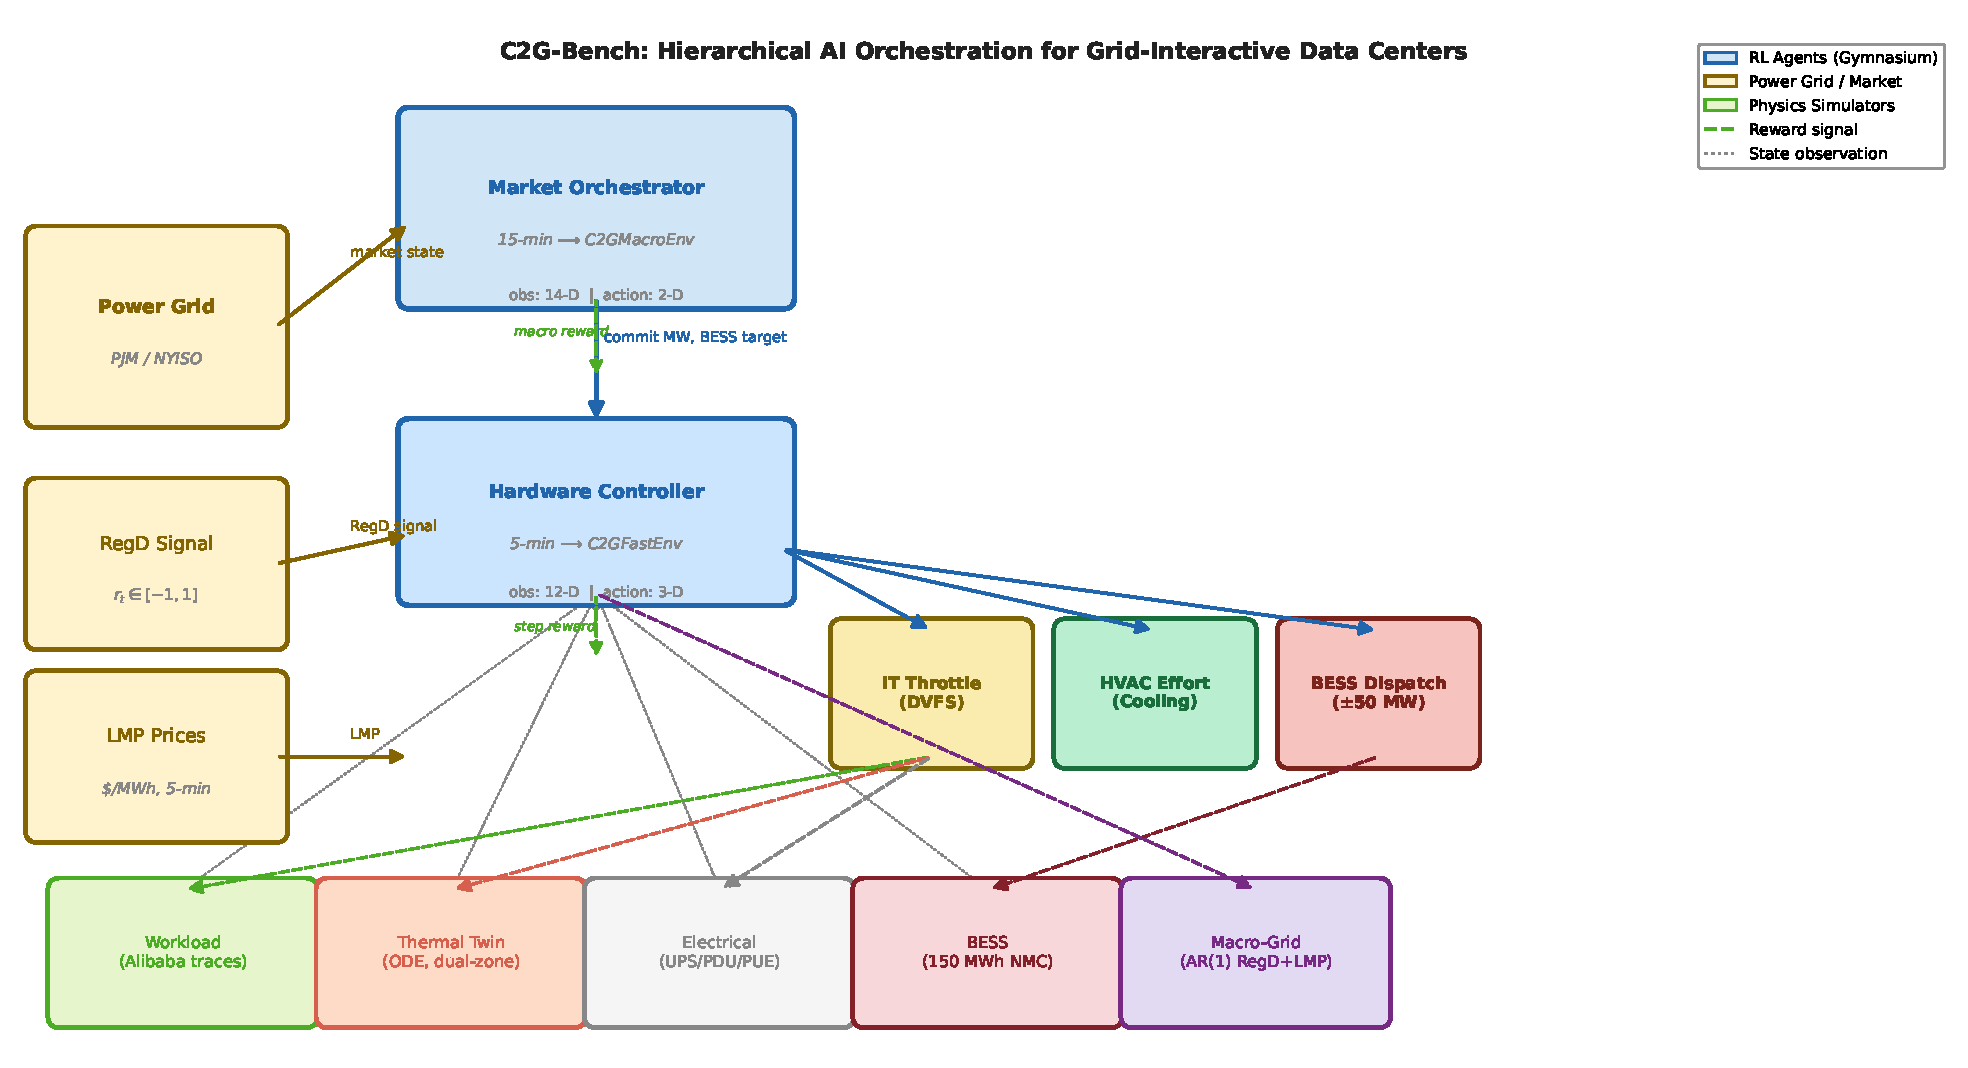
\includegraphics[width=\linewidth]{fig1_architecture.pdf}
  \caption{\cname{} hierarchical architecture. \envhigh{} sets 15-minute market
  commitments; \envlow{} executes 5-second hardware control across four physical
  levers and seven physics simulators.}
  \label{fig:architecture}
\end{figure}

\subsection{Data}
\label{sec:data}

\cname{} is driven by open-access datasets preprocessed into aligned
5-minute-resolution CSVs:

\begin{itemize}[leftmargin=*, itemsep=2pt]
  \item \textbf{Alibaba Batch v2023} (\texttt{batch\_v2023.csv}).
        33 days of GPU scheduling data~\citep{alibaba2023cluster}.
        We extract \texttt{gpu\_milli\_request} and normalise by the 99th
        percentile (12,620 milli-GPU) to get per-tick utilisation $u_{\text{batch}}$.
        78\% of ticks have zero arrivals, making this trace highly bursty.

  \item \textbf{Alibaba DLRM v2025} (\texttt{dlrm\_v2025.csv}).
        30 days of DLRM inference serving~\citep{alibaba2023cluster}.
        We extract \texttt{active\_gpu\_count} and normalise by 227 to
        get $u_{\text{dlrm}}$. This trace is continuous and predictable,
        with a clear diurnal pattern.

  \item \textbf{Alibaba GenAI v2026} (\texttt{genai\_v2026.csv}).
        288 ticks (one day) of LLM inference traffic, tiled cyclically.
        Ticks with \texttt{avg\_gpu\_duty\_cycle} above the 75th percentile
        (12.19\%) are flagged as spikes ($\mathbf{1}_{\text{spike}}$).
        About 25\% of ticks are in spike mode.

  \item \textbf{Energy load data.}
        Real zonal load from six ISOs (NYISO, PJM, CAISO, ERCOT, ENTSO-E, AEMO),
        converted to LMP through a load-duration proxy calibrated per market.

  \item \textbf{NOAA weather.}
        Hourly dry-bulb temperature from co-located weather
        stations~\citep{noaa2024isd}.
        For markets without local data, a calibrated two-harmonic synthetic
        model reproduces the correct seasonal and diurnal envelope.
\end{itemize}

All datasets are bundled under their original open-access licences.
Preprocessing scripts are in \texttt{preprocessing/}.

\subsection{Physical Simulators}
\label{sec:simulators}

\cname{} integrates seven independent, unit-tested physics engines running
at a canonical timestep of $\Delta t = 5$~s.
Each engine exposes a stateless \texttt{step()} method; the Gym environments
compose them at every tick.
All temporal dynamics use exact-exponential analytical solutions; no numerical
ODE solvers are used.

\paragraph{Workload Orchestrator.}
Models a 250~MW two-zone facility: 2,000 liquid-cooled GPU racks (Zone~A)
and 2,500 air-cooled CPU racks (Zone~B).
Rack power follows a superlinear utilisation model:
\begin{equation}
  P_{\text{rack}}(u) = P_{\text{idle}} + (P_{\max} - P_{\text{idle}})\,u^{\alpha},
  \label{eq:rack}
\end{equation}
with $\alpha_A = 1.4$ (GPU) and $\alpha_B = 1.2$ (CPU).
The three traces map to racks as follows:
batch v2023 drives 1,200 Zone~A racks ($P_{\text{flex}}$, throttleable via DVFS);
GenAI v2026 drives 800 Zone~A racks ($P_{\text{base,A}}$, rigid);
DLRM v2025 drives 2,500 Zone~B racks ($P_{\text{base,B}}$, rigid).
74\% of total IT power is rigid; the agent controls only the remaining 26\%
through batch throttling.
Unserved batch work defers into a FIFO queue tracked via Little's Law.

\paragraph{Thermal Twin.}
Models Zone~A and Zone~B as independent lumped-capacitance thermal masses
with exact-exponential integration:
\begin{equation}
  T_z(t{+}\Delta t) = T_{\text{eq}} + \bigl(T_z(t) - T_{\text{eq}}\bigr)\,
  e^{-K_{\text{tot}}\,\Delta t / C_z},
  \label{eq:thermal}
\end{equation}
where $T_{\text{eq}}$ is the equilibrium temperature given current heat input,
cooling, and ambient coupling.

Zone~A uses liquid cooling with a CDU pump speed action
$\omega_{\text{pump}} \in [0.15, 1]$ that controls effective conductance.
At minimum pump speed, the thermal time constant extends from $\approx$12.7~min
to $\approx$85~min, allowing the water loop to act as a short-horizon thermal
battery.
Zone~B uses air cooling with HVAC fan effort $u_{\text{hvac}} \in [0, 1]$.
Both zones share a safety limit of $T_{\text{safe}} = 35$\textdegree C (episode
termination) and warning threshold $T_{\text{warn}} = 33$\textdegree C (reward
penalty).

\paragraph{Electrical and Loss Model.}
Maps IT + cooling power to facility draw through three closed-form loss stages:
UPS (double-conversion, load-dependent efficiency), PDU (fixed 1.5--2.0\%),
and main transformer (iron + copper losses at 300~MVA).
Dynamic PUE is computed every tick as $\text{PUE}(t) = P_{\text{facility}} / P_{\text{IT}}$.

\paragraph{BESS Simulator.}
A 150~MWh / 50~MW NMC Li-ion battery with round-trip efficiency that degrades
with C-rate and SOC:
\begin{equation}
  \eta(C, \text{SOC}) = \max\!\bigl(0.70,\;
  \eta_{\text{peak}}^2 - k_C\,C^2 - k_{\text{SOC}}(\text{SOC} - 0.5)^2\bigr),
  \label{eq:bess}
\end{equation}
with $\eta_{\text{peak}} = 0.97$, $k_C = 0.008$, $k_{\text{SOC}} = 0.010$.
SOC is bounded to $[0.10, 0.95]$ with smooth power derating near limits.
Capacity fade accumulates linearly with throughput.

\paragraph{Macro-Grid Signal Generator.}
Produces two exogenous signals per tick, parameterised by a market preset
(Section~\ref{sec:markets}).
The regulation signal is an AR(1) process:
$r_t = \rho\,r_{t-1} + \varepsilon_t$, $\varepsilon_t \sim \mathcal{N}(0, \sigma^2)$,
with market-specific $\rho$ and $\sigma$.
A drift correction enforces energy neutrality over the settlement window.
The LMP uses a load-duration proxy calibrated per market.

\paragraph{Renewable Generator.}
Models 100~MW wind (IEC power curve) and 75~MW solar PV (PVUSA model)
with degradation, driven by the weather engine.

\paragraph{Weather Engine.}
Loads real NOAA ISD data or generates calibrated synthetic temperatures using
a two-harmonic model with per-market parameters (Table~\ref{tab:weather}).
Ambient temperature drives cooling COP and envelope heat gain.

\begin{figure}[t]
  \centering
  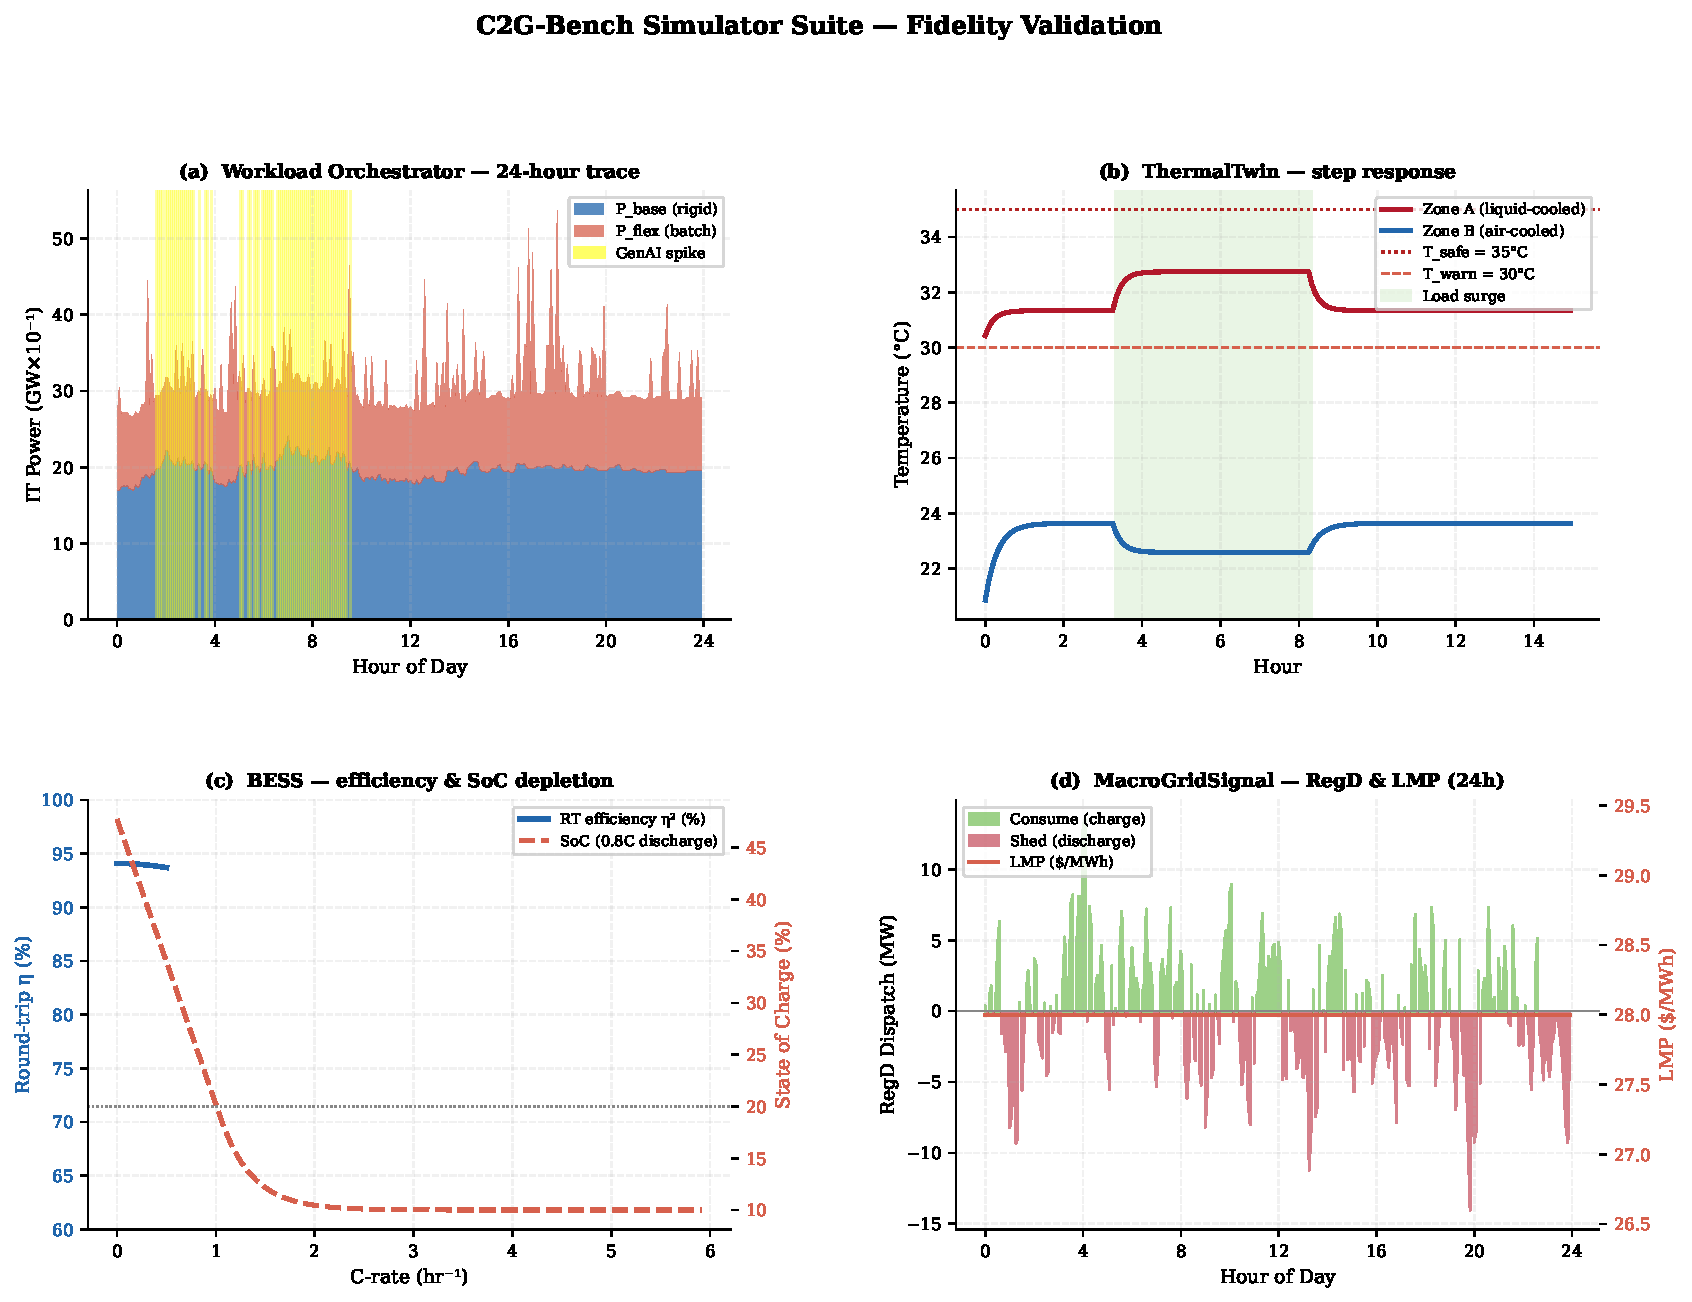
\includegraphics[width=\linewidth]{fig2_simulators.pdf}
  \caption{Simulator fidelity.
  (a)~24-hour IT power trace showing rigid $P_{\text{base}}$ and throttleable
  $P_{\text{flex}}$ with GenAI spikes.
  (b)~Zone~A and B step-response under a load surge.
  (c)~BESS efficiency vs C-rate and SOC depletion at 0.8C.
  (d)~RegD dispatch with NYISO LMP overlay.}
  \label{fig:simulators}
\end{figure}

\subsection{Supported Grid Markets}
\label{sec:markets}

\cname{} supports six ISO market configurations spanning three continents
(Table~\ref{tab:markets}).
Each preset encodes a distinct regulation product, AR(1) signal statistics,
LMP calibration, and settlement window.
The physical simulators, observation spaces, and reward functions are identical
across markets, enabling direct cross-market policy transfer studies.

\begin{table}[t]
\centering
\caption{Supported grid market presets.
$\rho$ and $\sigma$ are AR(1) parameters at the 5-second timestep.
LMP base and slope in USD/MWh.}
\label{tab:markets}
\small
\setlength{\tabcolsep}{4pt}
\begin{tabular}{llllrrrrl}
\toprule
\textbf{ID} & \textbf{ISO} & \textbf{Hub} & \textbf{Reg.\ product}
  & $\rho$ & $\sigma$ & \textbf{Base} & \textbf{Slope} & \textbf{Archetype} \\
\midrule
\texttt{nyiso\_nyc}   & NYISO   & New York City     & AGC Secondary  & 0.9963 & 0.022 & 28 & 18 & Baseline (real data) \\
\texttt{pjm\_dom}     & PJM     & Ashburn VA        & RegD fast AGC  & 0.9963 & 0.022 & 35 & 10 & Largest market \\
\texttt{caiso\_pgae}  & CAISO   & Bay Area          & REGU / REGD    & 0.9960 & 0.025 & 48 & 28 & Duck curve \\
\texttt{ercot\_north} & ERCOT   & Dallas-Fort Worth & ECRS           & 0.9950 & 0.030 & 28 & 55 & Isolated grid \\
\texttt{entso\_de}    & ENTSO-E & Frankfurt         & FCR-N          & 0.9980 & 0.015 & 60 &  8 & Deep EU market \\
\texttt{aemo\_nsw}    & AEMO    & Western Sydney    & Regulation FCAS & 0.9945 & 0.032 & 55 & 45 & High renewables \\
\bottomrule
\end{tabular}
\end{table}

\begin{table}[t]
\centering
\caption{Weather calibration per market.
SH = southern hemisphere (phase negated).
Src: R = real CSV, S = calibrated synthetic.}
\label{tab:weather}
\small
\setlength{\tabcolsep}{5pt}
\begin{tabular}{llrrrrl}
\toprule
\textbf{Market} & \textbf{Station} & $\bar{T}$ & $A_{\text{ann}}$ & $A_{\text{day}}$ & \textbf{Range} & \textbf{Src} \\
\midrule
\texttt{nyiso\_nyc}   & Central Park   & 13.0 & 12.5 & 5.0 & $[-20, 42]$ & R \\
\texttt{pjm\_dom}     & Reagan Natl    & 15.0 & 13.0 & 7.0 & $[-15, 42]$ & S \\
\texttt{caiso\_pgae}  & SJC Mineta     & 14.5 &  6.5 & 8.0 & $[-5,  42]$ & S \\
\texttt{ercot\_north} & DFW Intl       & 19.5 & 15.0 & 9.0 & $[-15, 46]$ & S \\
\texttt{entso\_de}    & Frankfurt FRA  & 11.0 & 10.5 & 7.0 & $[-20, 40]$ & S \\
\texttt{aemo\_nsw}    & Bankstown SH   & 18.5 &  9.0 & 8.0 & $[-5,  46]$ & S+SH \\
\bottomrule
\end{tabular}
\end{table}

\subsection{Gym Environments}
\label{sec:gym}

Both environments implement the Gymnasium interface~\citep{gymnasium2023}.
Observations are normalised to approximately $[-1,1]$ or $[0,1]$; actions are
clipped to their declared boxes before passing to simulators.

\paragraph{\envlow{} -- Low-Level (5-second).}

\textbf{Observation space} (17-D \texttt{Box}):
normalised Zone~A and B temperatures, SOC, base and flex IT load fractions,
facility power, regulation signal, LMP, grid load, GenAI spike flag,
previous throttle and pump actions, PUE, ambient temperature,
frequency deviation, PCC voltage, and batch queue backlog.

\textbf{Action space} (4-D \texttt{Box}):
(1)~DVFS throttle on batch workloads $\theta \in [0,1]$;
(2)~CDU pump speed $\omega_{\text{pump}} \in [0,1]$;
(3)~HVAC fan effort $u_{\text{hvac}} \in [0,1]$;
(4)~BESS dispatch $d_{\text{bess}} \in [-1,1]$ (charge to discharge).

\textbf{Reward function.}
At each 5-second tick:
\begin{equation}
  r_t = \alpha\,\theta
      - \beta\,\frac{|\deltap^{\text{dem}} - \deltap^{\text{act}}|}{P_{\text{norm}}}
      - \gamma\,\max(0, T_{\max} - T_{\text{warn}})
      - \delta_{\text{soc}}\,\mathbf{1}_{\text{soc}\notin[0.10,0.90]}
      - \delta_f\,\max(0,|\Delta f| - 0.2)
      - \delta_v\,\varepsilon_v
      - \delta_q\,q_{\text{backlog}},
  \label{eq:reward}
\end{equation}
with $\alpha{=}1$, $\beta{=}2$, $\gamma{=}5$,
$\delta_{\text{soc}}{=}2$, $\delta_f{=}2$, $\delta_v{=}5$, $\delta_q{=}2$.
The seven terms capture throughput, regulation tracking, thermal safety,
BESS health, frequency stability, voltage compliance, and SLA backlog.
The large coefficients on thermal ($\gamma$) and voltage ($\delta_v$) terms
force agents to treat these as hard constraints in practice.

\textbf{Episode:} 17,280 ticks (24 hours).
Early termination if $\max(T_A, T_B) \geq 35$\textdegree C,
$|\Delta f| \geq 0.5$~Hz, or $V_{\text{pcc}} < 0.90$~pu.

\paragraph{\envhigh{} -- High-Level (15-minute).}

\envhigh{} wraps \envlow{} in a temporal abstraction: each macro action
spans 180 sub-steps (one settlement interval).
The low-level environment is stepped 180 times using default actions derived
from the macro decision; a callback hook allows plugging in a learned
low-level policy for hierarchical evaluation.

\textbf{Action space} (2-D): regulation capacity commitment $c \in [0,1]$
and average BESS dispatch target $d \in [-1,1]$.
\textbf{Observation space} (17-D): interval-aggregated statistics of the
low-level observations, including thermal headroom, mean frequency deviation,
mean voltage, and batch backlog.
\textbf{Reward:} mean of 180 sub-step rewards plus an LMP dispatch bonus
($\mu_{\text{lmp}} = 0.1$) and commitment churn penalty ($\mu_c = 0.05$).

% ============================================================================
\section{Evaluation Scenarios}
\label{sec:scenarios}
% ============================================================================

\cname{} defines four scenarios that stress-test specific failure modes
(Table~\ref{tab:scenarios}).
All scenarios share the same simulator code; only initial conditions and
exogenous stressors differ.
Each scenario can be combined with any of the six markets, producing 24
distinct evaluation configurations.

\begin{table}[t]
\centering
\caption{Evaluation scenarios. All share the same simulators and reward weights.
dyn-$T$ = weather-driven ambient temperature.}
\label{tab:scenarios}
\small
\setlength{\tabcolsep}{3pt}
\begin{tabular}{llllrcrl}
\toprule
\textbf{ID} & \textbf{Name} & \textbf{Market} & $T_{\text{amb}}$ & \textbf{MW} & \textbf{Spike} & \textbf{dyn-$T$} & \textbf{Key stressor} \\
\midrule
\texttt{default}     & Baseline       & NYISO NYC   & 25\textdegree C & 15 & $1.0\times$ & \checkmark & Balanced operation \\
\texttt{scenario\_a} & GenAI Crisis   & PJM DOM     & 30\textdegree C & 20 & $1.8\times$ &            & Bursty GenAI + high commitment \\
\texttt{scenario\_b} & Thermal Squeeze & ERCOT North & 40\textdegree C & 30 & $1.0\times$ &            & Near-limit ambient \\
\texttt{scenario\_c} & Battery Drain  & AEMO NSW    & 32\textdegree C & 20 & $1.2\times$ &            & Low SOC (15\%), cooling fault \\
\bottomrule
\end{tabular}
\end{table}

\texttt{default} is the recommended starting point for algorithm development.
\texttt{scenario\_a} (GenAI Crisis) tests the conflict between IT throughput
and grid support when GenAI spikes consume the DVFS headroom.
\texttt{scenario\_b} (Thermal Squeeze) pushes ambient temperature to 40\textdegree C,
collapsing the thermal safety margin and degrading cooling COP by 30\%.
\texttt{scenario\_c} (Battery Drain) starts the BESS at 15\% SOC with a
simulated CDU pump degradation (60\% efficiency), forcing simultaneous
thermal and energy management under compound failure.

% ============================================================================
\section{Evaluation Metric Suite}
\label{sec:metrics}
% ============================================================================

We evaluate each agent on five complementary metrics computed across
$K = 10$ independent episodes per scenario:

\begin{itemize}[leftmargin=*, itemsep=2pt]
  \item \textbf{Tracking RMSE} (kW):
        $\sqrt{\frac{1}{T}\sum_t(\deltap_t^{\text{dem}} - \deltap_t^{\text{act}})^2}$.
        Primary grid service quality. Lower is better.
  \item \textbf{Thermal violation rate}: fraction of ticks with
        $\max(T_A, T_B) > T_{\text{warn}} = 33$\textdegree C.
  \item \textbf{Throughput ratio}: mean batch throttle $\bar{\theta}$.
        Higher is better (more compute served).
  \item \textbf{BESS degradation}: cumulative capacity fade $\times 10^4$.
        Captures long-term asset health.
  \item \textbf{Survival rate}: fraction of episodes completing the full
        17,280-tick horizon without thermal, frequency, or voltage termination.
\end{itemize}

The suite is deliberately non-reducible.
An agent with low tracking RMSE may achieve it by exhausting the BESS
(high degradation), or maintain high throughput by ignoring the regulation
signal (high RMSE).
These hidden trade-offs are only visible when the full suite is reported.

% ============================================================================
\section{Baseline Experiments}
\label{sec:experiments}
% ============================================================================

\subsection{Baselines}
\label{sec:baselines}

We evaluate four agents:

\paragraph{Random.}
Uniform random actions from the action space at each tick.
This is a lower bound on performance.

\paragraph{Rule-Based MPC.}
A hand-crafted threshold controller with four rules:
(1)~thermal protection (increase cooling when $T > T_{\text{warn}}$);
(2)~BESS dispatch proportional to the regulation signal with SOC guards;
(3)~DVFS fallback under low SOC;
(4)~opportunistic BESS charging during quiet periods.

\paragraph{PPO~\citep{schulman2017ppo}.}
On-policy actor-critic with a $[256, 256]$ MLP.
Trained for 300k steps over 4 parallel environments with VecNormalize.

\paragraph{SAC~\citep{haarnoja2018sac}.}
Off-policy maximum-entropy agent with automatic entropy tuning.
Trained for 200k steps with a replay buffer of $10^5$.

All agents use Stable-Baselines3~\citep{raffin2021stable}.
Experiments are configured through Hydra~\citep{hydra2019}; each run
saves a config snapshot, per-episode CSV, and TensorBoard events.

\subsection{Results}
\label{sec:results}

Table~\ref{tab:results_default} shows results on the \texttt{default}
scenario (3 seeds, mean reported).
Table~\ref{tab:results_cross} shows cross-scenario results.

\begin{table}[t]
\centering
\caption{Baseline results on \texttt{default} scenario (3 seeds, mean).
$\downarrow$ = lower is better; $\uparrow$ = higher is better.
\textbf{Bold} = best per column.}
\label{tab:results_default}
\small
\begin{tabular}{lrrrrr}
\toprule
\textbf{Agent} & \textbf{RMSE$\downarrow$} & \textbf{Viol.$\downarrow$} & \textbf{Surv.$\uparrow$} & \textbf{PUE$\downarrow$} & \textbf{Reward$\uparrow$} \\
 & (kW) & (rate) & (rate) & & \\
\midrule
Random         & 30,070 & 0.000 & 1.00 & 1.70 & $-2.93$ \\
Rule-Based MPC & 17,655 & 0.000 & 1.00 & 1.77 & $-0.78$ \\
PPO (300k)     &  4,235 & 0.000 & 1.00 & 1.97 & $+0.54$ \\
SAC (200k)     &  \textbf{476} & \textbf{0.000} & \textbf{1.00} & \textbf{1.68} & $\mathbf{+0.94}$ \\
\bottomrule
\end{tabular}
\end{table}

\begin{table}[t]
\centering
\caption{Cross-scenario results (3 seeds, mean). Scenario~B and C expose
systematic failures: PPO has high thermal violation rates and zero survival
on Scenario~C. SAC results for Scenario~C are pending.}
\label{tab:results_cross}
\small
\setlength{\tabcolsep}{3.5pt}
\begin{tabular}{llrrrr}
\toprule
\textbf{Scenario} & \textbf{Agent} & \textbf{RMSE$\downarrow$} & \textbf{Viol.$\downarrow$} & \textbf{Surv.$\uparrow$} & \textbf{Reward$\uparrow$} \\
\midrule
\multirow{4}{*}{A: GenAI Crisis}
 & Random     & 30,272 & 0.000 & 1.00 & $-2.09$ \\
 & Rule-Based & 16,480 & 0.000 & 1.00 & $-0.25$ \\
 & PPO        &  3,341 & 0.822 & 0.67 & $-0.67$ \\
 & SAC        &    \textbf{625} & \textbf{0.000} & \textbf{1.00} & $\mathbf{+0.95}$ \\
\midrule
\multirow{4}{*}{B: Thermal Squeeze}
 & Random     & 30,813 & 0.000 & 0.00 & $-1.96$ \\
 & Rule-Based & 14,359 & 0.000 & \textbf{1.00} & $+0.26$ \\
 & PPO        &  5,792 & 0.645 & 0.67 & $-3.04$ \\
 & SAC        &  \textbf{1,194} & \textbf{0.000} & \textbf{1.00} & $\mathbf{+0.94}$ \\
\midrule
\multirow{3}{*}{C: Battery Drain}
 & Random     & 28,628 & 0.000 & 0.33 & $-2.79$ \\
 & Rule-Based & 17,382 & 0.000 & \textbf{1.00} & $\mathbf{-0.39}$ \\
 & PPO        &  \textbf{4,317} & 0.539 & 0.00 & $-2.79$ \\
\bottomrule
\end{tabular}
\end{table}

\begin{figure}[t]
  \centering
  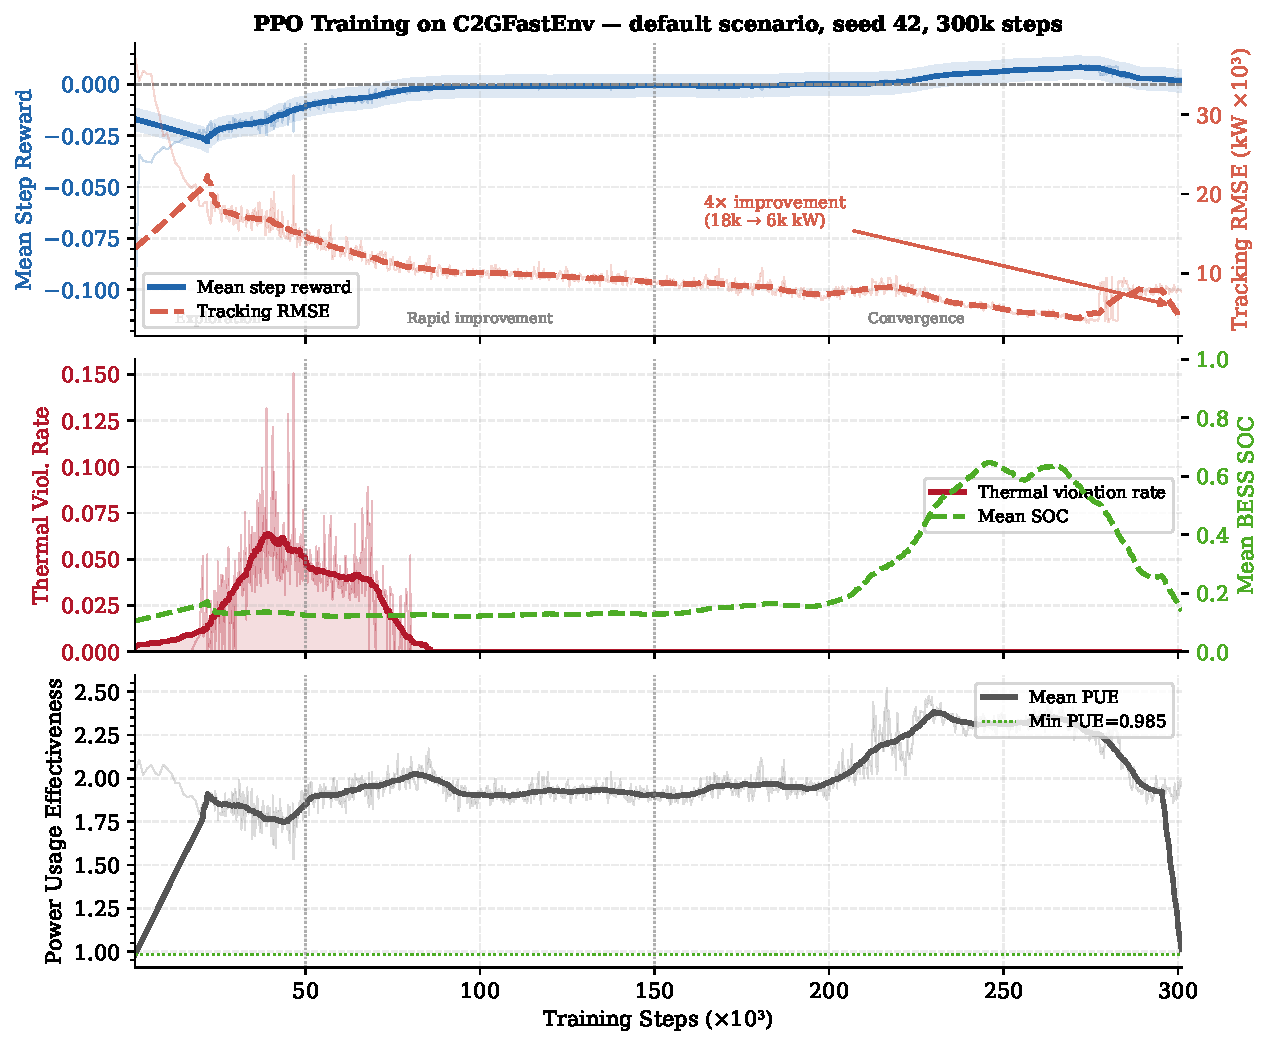
\includegraphics[width=\linewidth]{fig3_learning_curves.pdf}
  \caption{PPO training on \envlow{} (\texttt{default}, seed~42, 300k steps).
  Top: mean reward and tracking RMSE. RMSE drops from $\sim$33k to $\sim$8k~kW.
  Middle: thermal violation rate and mean SOC.
  Bottom: PUE converging toward 2.0.}
  \label{fig:learning_curves}
\end{figure}

\begin{figure}[t]
  \centering
  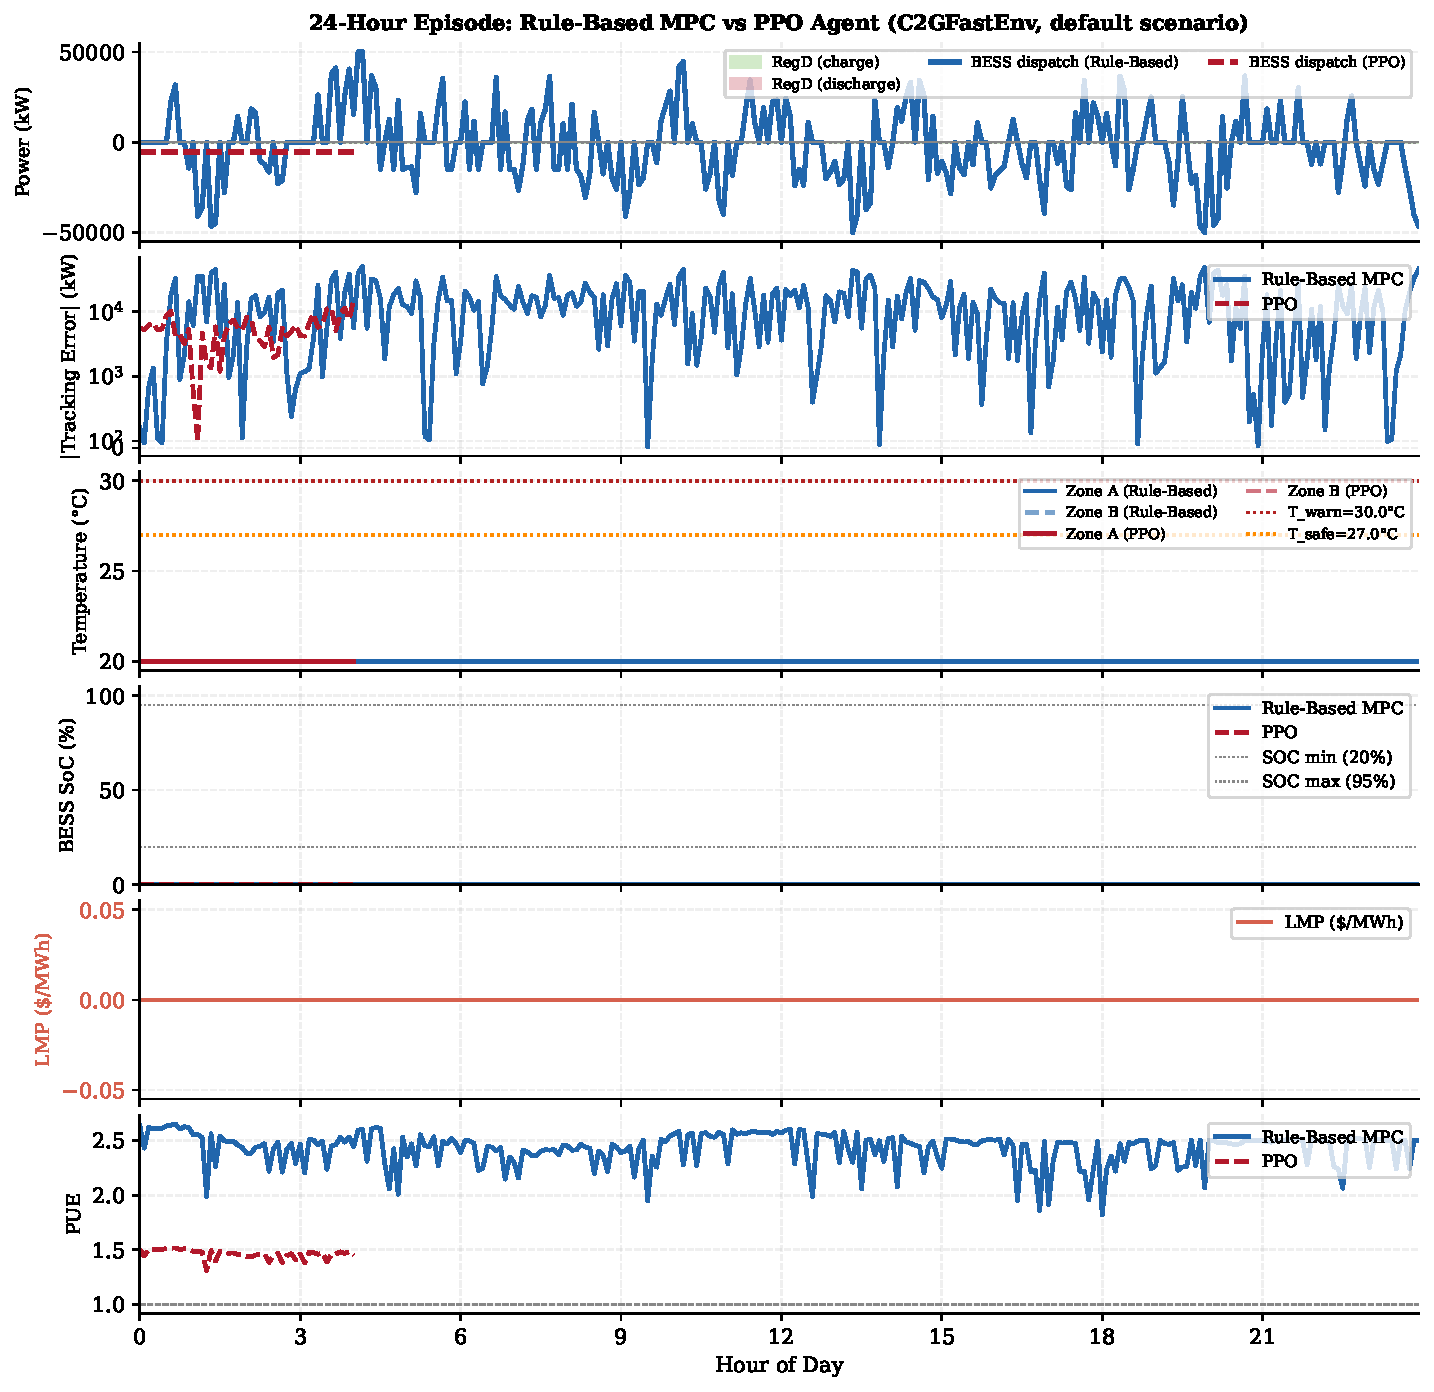
\includegraphics[width=\linewidth]{fig4_episode_trajectory.pdf}
  \caption{24-hour episode: Rule-Based MPC (blue) vs PPO (red).
  From top: RegD signal with BESS dispatch, tracking error (symlog),
  zone temperatures with safety thresholds, BESS SOC, LMP, PUE.}
  \label{fig:episode_trajectory}
\end{figure}

On the default scenario, SAC achieves a tracking RMSE of 476~kW, which is
37$\times$ lower than Rule-Based MPC (17,655 kW) and 9$\times$ lower than
PPO (4,235 kW).
All four agents survive the full episode and have zero thermal violations
under nominal conditions.

The stress scenarios reveal a different picture.
On Scenario~A (GenAI Crisis), PPO develops a thermal violation rate of 82\%
and survives only 67\% of episodes, while SAC maintains zero violations and
full survival.
On Scenario~B (Thermal Squeeze at 40\textdegree C), PPO has 65\% violations
and the random agent never survives.
On Scenario~C (Battery Drain), PPO has zero survival rate, terminating
early in every run due to thermal faults under the compound stress of low
SOC and degraded cooling.
Rule-Based MPC survives all scenarios but achieves high tracking RMSE
(14--18k~kW), showing that survival and regulation quality are competing
objectives.

These results demonstrate the value of the non-reducible metric suite:
PPO optimises for low RMSE but does so at the cost of thermal safety on
harder scenarios; Rule-Based MPC is safe but tracks poorly; SAC finds
a better balance but was not tested on Scenario~C at submission time.

\subsection{Failure Mode Analysis}
\label{sec:failures}

\paragraph{GenAI Crisis (Scenario~A).}
The 1.8$\times$ spike scale exhausts the DVFS throttle budget.
Agents that do not account for SOC trajectory exhaust the battery in the
first half and face uncovered regulation gaps in the second half.

\paragraph{Thermal Squeeze (Scenario~B).}
At 40\textdegree C ambient, the thermal safety margin collapses.
Rule-Based MPC overreacts by maximising cooling and zeroing throttle,
causing throughput collapse.
PPO learns a more nuanced trade-off but requires $>$150k steps to stabilise.

\paragraph{Battery Drain (Scenario~C).}
Starting at 15\% SOC with a cooling fault ($K_z \times 0.6$) forces
simultaneous thermal and energy management.
PPO terminates early in all runs, showing that current single-level
policies cannot jointly manage these constraints.
This motivates hierarchical agents that reason over both timescales.

% ============================================================================
\section{Reproducibility}
\label{sec:reproducibility}
% ============================================================================

\cname{} supports full experimental reproducibility:

\begin{enumerate}[leftmargin=*, itemsep=2pt]
  \item \textbf{Dependency management:} \texttt{uv sync} reproduces the exact
        environment from \texttt{pyproject.toml} and \texttt{uv.lock}.
  \item \textbf{Config snapshots:} Hydra stores config and override files
        in every output directory.
  \item \textbf{Seeded randomness:} all environments, policies, and signal
        generators accept an integer seed. Results are deterministic given
        the seed.
  \item \textbf{Test suite:} 493 pytest tests covering all simulators,
        environments, baselines, and CLI smoke tests.
  \item \textbf{Croissant metadata:} dataset lineage and RAI documentation
        (to be finalised with DOI at camera-ready).
\end{enumerate}

% ============================================================================
\section{Limitations and Future Work}
\label{sec:limitations}
% ============================================================================

\paragraph{Simulator fidelity.}
The thermal model is a lumped single-mass per zone. Real data centres have
spatial temperature gradients that this does not capture.
The BESS uses empirical efficiency curves, not electrochemical first-principles.

\paragraph{Scale context.}
The benchmark models a 250~MW hyperscale facility. Results may not transfer
to edge or colocation data centres with different cooling architectures
and workload mixes.

\paragraph{Market model.}
The AR(1) regulation signal is a simplified approximation of real RegD/AgC
signals. Future work should integrate live ISO API feeds for more realistic
evaluation.

\paragraph{Communication latency.}
The benchmark does not model communication delays between the market agent
and hardware controller, nor grid topology or congestion.

\paragraph{Multi-agent.}
The callback hook in \envhigh{} enables two-agent hierarchical evaluation,
but a fully cooperative multi-agent formulation (e.g., one agent per rack
row) is left for future work.

\paragraph{Hardware-in-the-loop.}
All results are simulation-only. Validation against real hardware is needed
before any deployment.

% ============================================================================
\section{Broader Impact}
\label{sec:impact}
% ============================================================================

\cname{} is intended to benefit research at the intersection of reinforcement
learning and sustainable energy infrastructure.

\paragraph{Grid decarbonisation.}
Data centres that accurately track regulation signals reduce the need for
fossil-fuel peaker plants. Even modest improvements in tracking RMSE at
250~MW scale translate to meaningful reductions in grid carbon intensity
during stress events.

\paragraph{AI infrastructure efficiency.}
By including SLA backlog in the reward and survival rate in the evaluation,
\cname{} incentivises agents that preserve compute throughput while providing
grid services.

\paragraph{Misuse risks.}
The benchmark is for scientific evaluation, not direct deployment.
Policies trained in simulation must be validated against real hardware
before any grid-interactive use.
We do not foresee meaningful negative consequences from releasing this
benchmark.

% ============================================================================
\section{Conclusion}
\label{sec:conclusion}
% ============================================================================

We presented \cname{}, a cyber-physical evaluation benchmark for hierarchical
RL in grid-interactive hyperscale data centres.
The benchmark combines seven physics engines, two Gymnasium environments at
coupled timescales (\envlow{} at 5~s, \envhigh{} at 15~min),
17-dimensional observations, a seven-component reward, six ISO market
configurations, four stress scenarios, and a five-metric non-reducible
evaluation suite.
A Simplex-architecture safety shield enforces hard constraints as a plug-in
layer for any agent.

Baseline results with Random, Rule-Based MPC, PPO, and SAC show that the
default scenario is solvable (SAC achieves 476~kW tracking RMSE), but the
stress scenarios expose systematic failure modes.
PPO fails on Scenario~C (Battery Drain) with zero survival rate.
Rule-Based MPC survives all scenarios but tracks poorly (14--18k~kW RMSE).
These gaps establish concrete targets for future HRL research: agents that
jointly reason over thermal, energy, and grid-stability constraints across
the two timescales.

% ============================================================================
\section*{License and Code Availability}
\label{sec:license}
% ============================================================================

\cname{} is released under the Apache~2.0 License.
Source code, environments, simulators, and preprocessing scripts are available
at \url{https://github.com/antonio-guillen/c2g-bench-neurips2026}.
The Alibaba traces are redistributed under their original
terms~\citep{alibaba2023cluster};
NYISO data under the NYISO policy~\citep{nyiso2024lmp};
NOAA ISD data is in the public domain~\citep{noaa2024isd}.
No personally identifiable information is in any dataset.

\bibliographystyle{plainnat}
\bibliography{references}

\end{document}
